\section{Implementación firmware}

En este capítulo se expone el trabajo relacionado con la programación a bajo nivel realizada sobre la electrónica propuesta en el capítulo Módulo Hardware.
Dado que la electrónica se basa en la plataforma Arduino, tal programación se realiza usando su propio lenguaje,  implementado en C/C++.

Este lenguaje se llama \textbf{Wiring} y se define a sí mismo como:

\textit{Entorno de programación de entradas/salidas de código abierto para explorar las artes electrónicas, los medios materiales, la enseñanza y el aprendizaje de la programación informática y creación de prototipos con electrónica.
}


\subsection{Diseño y Análisis}

Pasamos a determinar los requisitos que debe satisfacer nuestro firmware.
El requisito principales es claro, y consiste en ser capaz de controlar y manejar toda la información todos los periféricos  los datos que arrojan, ello se puede desglosar:

\begin{itemize}
	\item \textbf{Motor}, controla el movimiento, la velocidad, y la posición. 
	\item \textbf{Botones y potenciometos}, controla las pulsaciones y el cambio en el valor de los potenciometros, para controlar el dispositivo de forma manual. 
	\item \textbf{Pantalla LCD}, mostrar toda la información por pantalla.
	\item \textbf{Sensores}, recabar información del estado del dispositivo, temperatura, fines de recorrido.
	\item \textbf{Sesión persistente}, almacenar información de trabajo a otra.
	\item \textbf{API Serie}, interpretar y manejar comando vía mediante comunicación puerto serie, para permitir controlar el dispositivo desde un host.
\end{itemize}

Todo ello debe implementarse con una buena calidad permitiendo añadir más módulos y que se pueda cambiar fácilmente el repertorio de instrucciones de la API.

\subsection{Arquitectura firmware}


Para la programación del firmware sigo un diseño donde diferencio 4 bloques.


\begin{itemize}
	\item \textbf{Initializer}: Método \textbf{init} de la api de Arduino, que se ejecuta en primera instancia, prepara todo el entorno de ejecución, declarando las entradas, salidas,  reservando memoria, iniciar interrupciones, así como ejecutar rutinas como cargar sesión anterior o crear instancias a modo de singleton para manejador los diferentes periféricos. 
	\item \textbf{Controlador principal}: Bucle principal que se ejecuta periódicamente (el periodo no se puede modificar y lo marca la velocidad del reloj del micro), por lo tanto no es adecuado ejecutar rutinas con restricciones temporales fuertes, se corresponde con el método \textbf{loop}, se ocupa de manejar la mayoria de las entradas y salidas.
	\item \textbf{Interrupciones software}, se ejecutan en un periodo marcado por un timer, similar al loop pero con periodos fijo, se usa para rutinas con restricciones temporales fuertes.
	item \textbf{Interrupciones hardware}, se ejecutan rutinas ligadas directamente a eventos de entrada y salida en alguno de los pines habilitados para tal fin. 
\end{itemize}

Podemos ver un diagrama simplificado en la siguiente imagen.

\begin{figure}
\centering
\includegraphics[width=0.7\linewidth]{"../images/Arquitectura firmware"}
\caption{}
\label{fig:Arquitecturafirmware}
\end{figure}

\subsection{Módulo motores}

Para el control del motor, dado que debemos hacerlo con una gran precisión, hacemos uso de la libreria 
\textbf{AccelStepper} \cite{accelstp} 

\subsection{Módulo control remoto}

Para realizar el control remoto, hago uso de la comunicación serie que incorpora la placa Arduino.


El puerto serie envía la información mediante una secuencia de bits. Para ello se necesitan al menos dos conectores para realizar la comunicación de datos, RX (recepción) y TX (transmisión). 

En ocasiones veréis referirse a los puertos de serie como UART. La UART (universally asynchronous receiver/transmitter) es una unidad que incorporan ciertos procesadores, encargada de realiza la conversión de los datos a una secuencia de bits y transmitirlos o recibirlos a una velocidad determinada.

Los puertos serie están físicamente unidos a distintos pines, en Arduino UNO y Mini Pro los pines empleados son 0 (RX) y 1 (TX).


\begin{lstlisting}[language=C, caption={Ejemplo lectura y escritura puerto serie},label={lst:write_read_serial_port_sample}]

void setup(){
Serial.begin(9600);
}

void loop(){

}

void witeCharapter(char c){
Serial.println(c);
}

void readCharapter(){
if (Serial.available()>0){
input=Serial.read();
Serial.println(input);
}


\end{lstlisting}


Dado que tengo una cantidad de funciones a ejecutar mediante comandos, necesito formalizar un protocolo basado en mensajes preestablecidos. \\
Por seguir una nomenclatura, todos los comandos tienen el siguiente formato: \\


$ COMANDO?ARGUMENTO1?ARGUMENTO2  $

Y a continuación una lista de los comandos utilizados.


\begin{figure}[h]
	\centering
	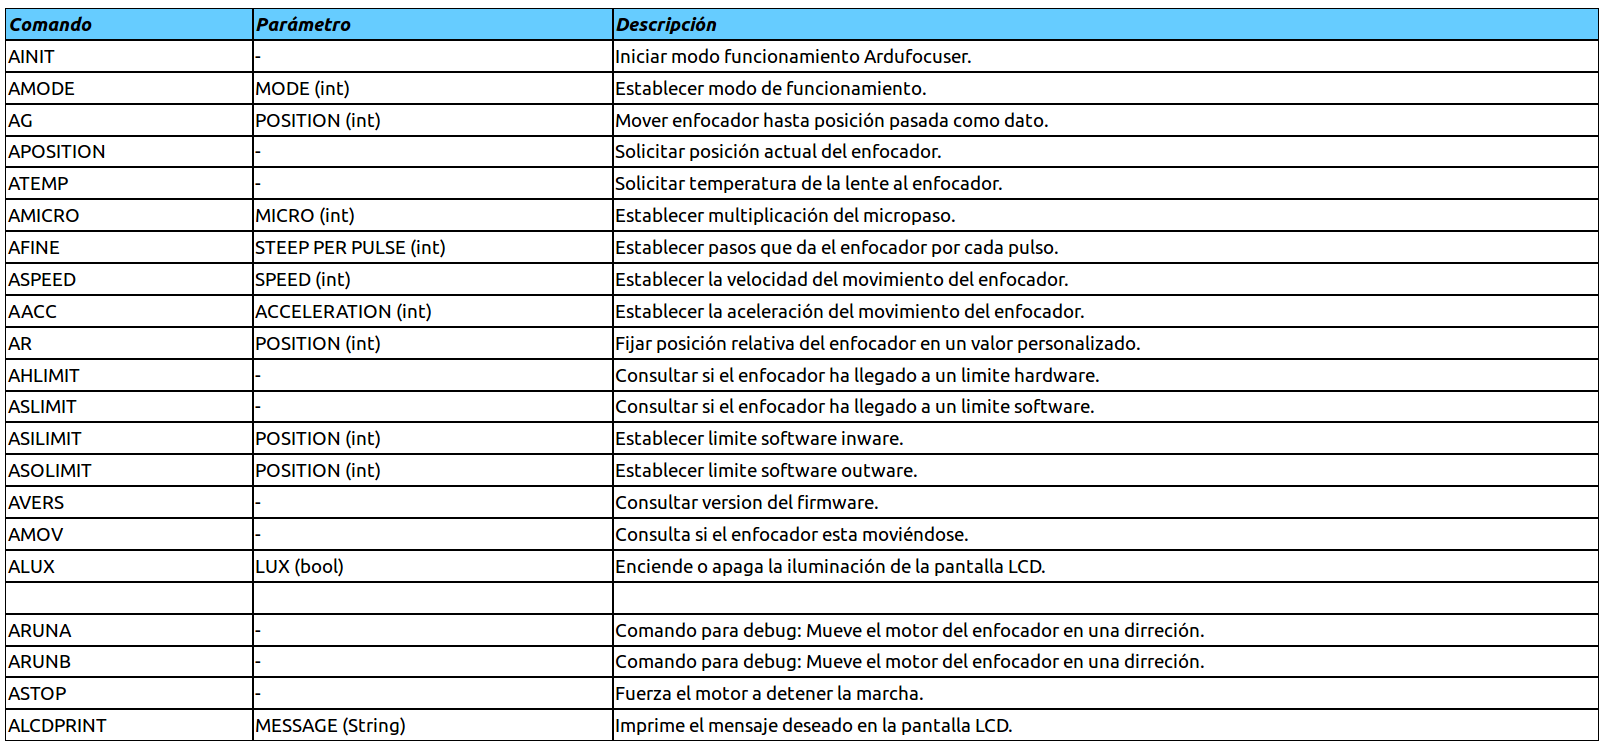
\includegraphics[width=1.1\linewidth]{../images/comando_ardufocuser}
	\caption{}
	\label{fig:comando_ardufocuser}
\end{figure}

Por regla general, todo comando tiene un mensaje de respuesta, bien indicando el nuevo estado del sistema que se ha cambiado (comandos escritura), bien información sobre el estado sobre el que solicitamos información (comandos lectura) o un ECHO del comando en algún otro caso.

\newpage


Con la experiencia y el trabajo, voy familiarizándome con la plataforma, conozco nuevas bibliotecas que me ayudan, nuevos periféricos,  así como mediante sesiones de refactorización, se consigue hacer código mantenible y modular. 

Es importante mencionar el uso de la herramienta \textbf{PlatformIO}, que se define a sí misma como un ecosistema abierto de desarrollo orientado a hardware. 


Tres son las características más sustanciales. 


- PlatformIO IDE: Un IDE orientado a la programación hardware, con funciones para facilitar la depuración, así como avisos para mejorar la calidad, totalmente configurado para compilar y cargar el programa directamente en una placa física, o en una placa virtual.

\begin{figure}
	\centering
	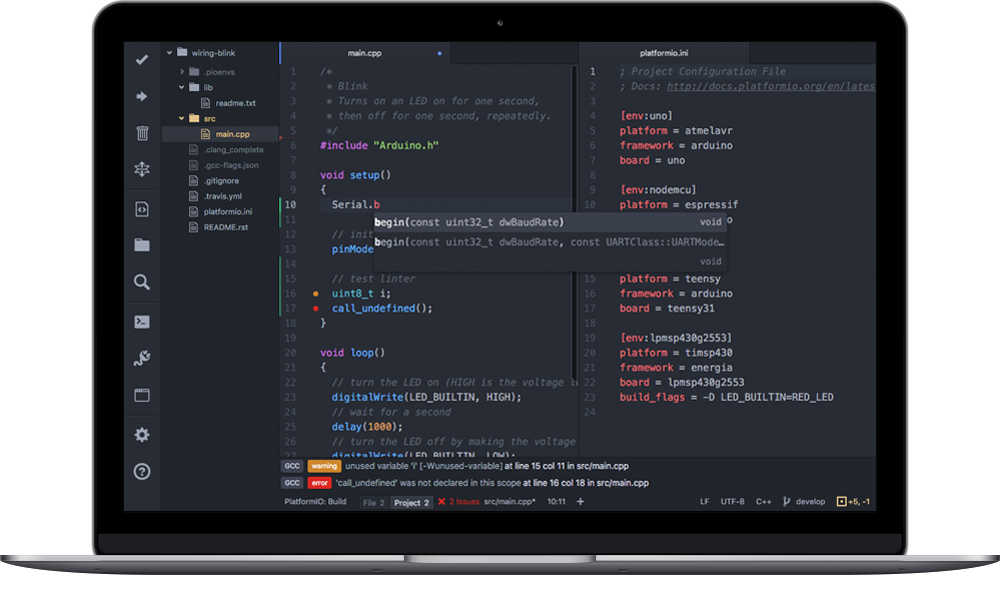
\includegraphics[width=0.7\linewidth]{../images/ide_arduino}
	\caption{}
	\label{fig:ide_arduino}
\end{figure}

- Terminal para realizar compilación en el cloud  para diferentes placas, así como permite compilación desde plataformas de integración continua como Travis CI.

- Gestor de bibliotecas y dependencias, tiene un repositorio con las bibliotecas más usadas, pudiendo buscar y actualizar rápidamente. 



El código fuente del firmware queda distribuido en los siguientes ficheros.

\begin{itemize}
	
\item $Ardufocuser-config.h$: Encapsula gran parte de la configuración, así como el mapeo de pines y demás definiciones. 
\item $Ardufocuser-init.h$: Inicializa el sistema, creando las instancias de los objetos utilizados, variables globales, contadores y demás estados.
\item $Ardufocuser-cmd.h$: Se definen los comandos remotos, junto con sus funciones callback asociadas.
\item $Ardufocuser-utils.h$: Incorpora algunas funciones de propósito general útiles en algunos de los módulos. 
\item $Ardufocuser.ino$: Es el script principal, incluye los ficheros anteriores, contiene las funciones setup(),  loop() y callback de las interrupciones hardware y software.

\item $library.json$: Hace referencia a las librerías de terceros, catalogadas, y con referencias al sitio web y al desarrollador o equipo de desarrollo. Por seguridad también las incorporo al repositorio en el directorio libs.  


\end{itemize}
\newpage
\begin{lstlisting}[language=C, caption={Núcleo implementación firmware  ardufocuser},label={lst:nucleo_firmware_ardufocuser }]

	void setup()
	{
		//Inicia comunicación serie.
		Serial.begin(9600);
		
		// Inicia pantalla LCD.
		lcd.begin();
		lcd.backlight();
		
		// Saludo inicial.
		welcome("   ARDUFOCUSER  ");
		
		// Velocidad y Aceletación inicial del motor.
		motor.setMaxSpeed(200);
		motor.setAcceleration(1000);
		
		//Iniciamos control Nunckuck
		chuck.begin();
		chuck.update();
		
		// Actualizamos con datos guardados en sesion anterior
		load_session();
		
		// Iniciamos interrupciones Software.
		// Gestiona movimiento del motor.
		Timer1.initialize(50);
		Timer1.attachInterrupt(timerFunction);
		
		// Inicia interrupciones hardware a la escucha.
		attachInterrupt ( 0, finA,RISING);
		attachInterrupt ( 1, finB,RISING);
		
		// Registramos y iniciamos comandos serie.
		registerCommand();
	}
	
	void loop()
	{
		// Leemos nuevo comando serie.
		serial_cmd.readSerial();
		
		// Leemos control manual y sensores auxiliares.
		read_manual_controller();
		
		// Actualizamos LCD.
		update_lcd_display();
		
		// Leemos controles nunchuck.
		nunckuck_controller();
		
		// Almacenamos estados de forma persistente 
		// para otra sesión.
		save_current_session();
	}



\end{lstlisting}


\section{Pruebas}

Además para asegurar que el firmware implementado, permite ser compilado en las distintas placas hacemos uso del framework   \textbf{PlatformIO} \cite{patform}.


- Buscador centralizado de bibliotecas, en los proyectos Arduino es uno de los problemas, dado que cada una de ellas puede provenir de una fuente totalmente diferente, con esta herramienta contamos con un solo lugar.

\newpage
\begin{lstlisting}[language=python, caption={Script travis para realizar integración continua},label={lst:write_read_serial_port_sample}]

language: python
python:
- "2.7"

install:
- python -c "$(curl -fsSL https://raw.githubusercontent.com/platformio/platformio/master/scripts/get-platformio.py)"
- wget https://github.com/josemlp91/ardufocuser_firmware/raw/master/Ardufocuser/libs/TimerOne.zip
- unzip TimerOne.zip
- wget https://github.com/josemlp91/ardufocuser_firmware/raw/master/Ardufocuser/libs/i2clcd.zip
- unzip i2clcd.zip
- wget https://github.com/josemlp91/ardufocuser_firmware/raw/master/Ardufocuser/libs/AccelStepper-1.49.zip
- unzip AccelStepper-1.49.zip
- wget https://github.com/josemlp91/ardufocuser_firmware/raw/master/Ardufocuser/libs/nunchuck.zip
- unzip nunchuck.zip

script:
- platformio ci Ardufocuser --lib="TimerOne" --lib="i2clcd" --lib="nunchuck" --lib="AccelStepper" --board=uno

\end{lstlisting}

